\documentclass{article}


\usepackage{amsmath, amsthm, amssymb, amsfonts}
\usepackage[makeroom]{cancel}
\usepackage{xcolor}
\usepackage{graphicx}
\usepackage{geometry}
\usepackage[american, RPvoltages]{circuitikz}

\usepackage{IEEEtrantools}

\usepackage{hyperref}
\usepackage[utf8]{inputenc}
\usepackage[english]{babel}

\geometry{
    textheight=9in,
    textwidth=6.5in,
    top=1in,
    headheight=12pt,
    headsep=25pt,
    footskip=30pt
}

\newcommand{\smallsignal}[2]{\lowercase{#1}_{\lowercase{#2}}}
\newcommand{\equationname}{Equation}

\newcommand{\cancelRed}[1]{\textcolor{red}{\cancel{\textcolor{black}{#1}}}}
\newcommand{\cancelToOne}[1]{\textcolor{red}{\cancelto{1}{\textcolor{black}{#1}}}}
\newcommand{\cancelToZero}[1]{\textcolor{red}{\cancelto{0}{\textcolor{black}{#1}}}}

\begin{document}

% ------------------------------------------------------------------------------
% Cover Page and ToC
% ------------------------------------------------------------------------------

\title{\textbf{\uppercase{Constant Power Load Harmonics}}}
\date{}
\author{\textbf{Eric Ponce} \\
		Massachusetts Institute of Technology}

\maketitle

% \tableofcontents

% ------------------------------------------------------------------------------

\section{Introduction}

This paper demonstrates the inherent presence of current harmonics in constant power loads driven by voltage pertubations.
It also presents a solution for the fourier series of the current, and compares it to the standard small signal model.
The circuit may be described as follows:

\begin{figure}[htbp]
\center
\begin{circuitikz}
	\draw (2, 0) node[ground]{};
	\draw (2, 0) -- ++(-2, 0)
		to[vsource, v=$V_T$] ++(0, 2)
		to[vsourcesin, v=$v_t$] ++(0, 2) -- ++(4, 0)
		to[generic,l=P] ++(0, -4) -- ++(-2, 0);
\end{circuitikz}
\caption{Constant Power Load Test Circuit.}
\end{figure}

Consider a load that draws constant power $P$ being driven by a voltage $v_T(t) = V_T + v_t\cos{t}$ where $V_I$ is the bias voltage and $v_i$ is the pertubation amplitude.
The current for this circuit is

\begin{equation}
i_T = \frac{P}{v_T(t)} = \frac{P}{V_T + v_t \cos{t}}.
\end{equation}

This \emph{is} a nonlinear function and contains harmonics at multiples of the fundamental which are neglected by traditional small signal approximation approaches.

Much past work has presented small-signal modeling approaches, but few consider the harmonics produced by constant power loads. 
Jesse Paul used Volterra Kernels to determine harmonics in constant power loads within real world systems and perform large-signal stability analysis \cite{leonard_2014}.

\newpage
\section{Fourier Series}

To solve for the fourier coefficients of the constant power load current, we start with a reminder of the definition of the fourier coefficients of a function $s(x)$ with a period of $2\pi$:

\begin{IEEEeqnarray}{rCl}
	A_0 &=& \frac{1}{2\pi} \int_{-\pi}^{\pi} s(x)\,dx \\
	A_n &=& \frac{1}{\pi} \int_{-\pi}^{\pi} s(x) \cos(nx)\,dx \\
	B_n &=& \cancelToZero{\frac{1}{\pi} \int_{-\pi}^{\pi} s(x) \sin(nx)\,dx}
\end{IEEEeqnarray}

Because the current is an even function, the $B_n$ coefficients will be zero. 
Before we begin to solve for the rest of the coefficients, we present the current in a more useful exponential form:

\begin{equation}
i_T = \frac{P}{v_T(t)} = \frac{P}{V_T + v_t \cos{t}} = \frac{P}{V_T + \frac{v_t}{2}(e^{jt}+e^{-jt})} = \frac{2P}{2V_T + v_t(e^{jt}+e^{-jt})}
\end{equation}

\subsection{DC Coefficient}

We can compute $A_0$ as follows using a substitution of $z=e^{jt}$ to convert it into a contour integral, followed by the use of the residue theorem around one of the poles:

\begin{IEEEeqnarray}{rCl}
A_0 &=& \frac{1}{2\pi} \int_{-\pi}^{\pi} \frac{2P}{2V_T + v_t(e^{jt}+e^{-jt})} dt \nonumber\\
	&=& \frac{P}{j\pi} \oint \frac{1}{z} \frac{1}{2V_T + v_t(z+z^{-1})} dz \nonumber\\
	&=& \frac{P}{jv_t\pi} \oint \frac{1}{z^2 + \frac{2V_T}{v_t}z + 1} dz \nonumber\\
	&=& \frac{P}{jv_t\pi} 2\pi j \mathop{\mathrm{Res}}_{z=z_0} \left(\frac{1}{z^2 + \frac{2V_T}{v_t}z + 1}\right) \nonumber\\
	&=& \frac{2P}{v_t} \mathop{\mathrm{Res}}_{z=z_0} \left(\frac{1}{(z-z_0)(z-z_1)}\right).
\end{IEEEeqnarray}

where $z_0$ and $z_1$ are the poles of the function and can be found using \eqref{eq:poles}.
The residue for this function is found by taking the limit:

\begin{IEEEeqnarray}{rCl}
\mathop{\mathrm{Res}}_{z=z_0} \left(\frac{1}{(z-z_0)(z-z_1)}\right) &=& \lim_{z\rightarrow z_0} \left(\frac{z-z_0}{(z-z_0)(z-z_1)}\right) \nonumber\\
	&=& \lim_{z\rightarrow z_0} \left(\frac{1}{(z-z_1)}\right) \nonumber\\
	&=& \frac{1}{(z_0-z_1)}
\end{IEEEeqnarray}

Finally, we arrive at the coefficient using \eqref{eq:pole_identity1}:

\begin{equation}
A_0 = \frac{2P}{v_t} \mathop{\mathrm{Res}}_{z=z_0} \left(\frac{1}{z^2 + \frac{2V_T}{v_t}z + 1}\right) = \frac{2P}{v_t} \frac{1}{2\sqrt{\left(\frac{V_T}{v_t}\right)^2 - 1}} = \frac{P}{\sqrt{V_T^2 - v_t^2}}.
\end{equation}

\subsection{Harmonic Coefficients}

We can compute $A_n$ as follows using a substitution of $z=e^{jt}$ and the same definitions of $z_0$ and $z_1$ as above:

\begin{IEEEeqnarray}{rCl}
A_n &=& \frac{1}{\pi} \int_{-\pi}^{\pi} \frac{2P \frac{e^{jnt}+e^{-jnt}}{2}}{2V_T + v_t(e^{jt}+e^{-jt})} dt \nonumber\\
	&=& \frac{P}{j\pi} \oint \frac{1}{z} \frac{z^n+z^{-n}}{2V_T + v_t(z+z^{-1})} dz \nonumber\\
	&=& \frac{P}{j\pi v_t} \oint \frac{1}{z^n}\frac{1+z^{2n}}{(z-z_0)(z-z_1)} dz \nonumber\\
	&=& \frac{2P}{v_t} \left(\mathop{\mathrm{Res}}_{z=z_0} \left(\frac{1}{z^n}\frac{1+z^{2n}}{(z-z_0)(z-z_1)}\right) + \mathop{\mathrm{Res}}_{z=0} \left(\frac{1}{z^n}\frac{1+z^{2n}}{(z-z_0)(z-z_1)}\right) \right).
\end{IEEEeqnarray}

Let's start with the residue at $z=z_0$:

\begin{equation}
\mathop{\mathrm{Res}}_{z=z_0} \left(\frac{1}{z^n}\frac{1+z^{2n}}{(z-z_0)(z-z_1)}\right) = \lim_{z\rightarrow z_0} \left(\frac{1+z^{2n}}{z^n (z-z_1)}\right) = \frac{1+z_0^{2n}}{z_0^n (z_0-z_1)}
\end{equation}

For the the residue at $z=0$, we use \eqref{eq:pole_identity3} and \eqref{eq:residue_identity2}:

\begin{IEEEeqnarray}{rCl}
	\mathop{\mathrm{Res}}_{z=0} \left(\frac{1}{z^n}\frac{1+z^{2n}}{(z-z_0)(z-z_1)}\right) &=& \mathop{\mathrm{Res}}_{z=0} \left(\frac{1+z^{2n}}{z^n}\frac{1}{z_0 - z_1}\sum_{k=0}^\infty z^k\left(z_0^{k+1} - z_1^{k+1}\right)\right) \nonumber\\
	&=& \lim_{z\rightarrow z_0} \left(\frac{1}{z^n}\frac{z}{z_0 - z_1}\left.\left(\sum_{k=0}^\infty z^k\left(z_0^{k+1} - z_1^{k+1}\right)\right)\right\vert_{k=n-1}\right) \nonumber\\
	&=& \lim_{z\rightarrow z_0} \left(\frac{1}{z^n}\frac{z}{z_0 - z_1}\left(z^{n-1} \left(z_0^{n} - z_1^{n}\right)\right)\right) \nonumber\\
	&=& \lim_{z\rightarrow z_0} \left(\frac{1}{z_0 - z_1}\left(z_0^{n} - z_1^{n}\right)\right) \nonumber\\
	&=& \frac{\left(z_0^{n} - z_1^{n}\right)}{z_0 - z_1}
\end{IEEEeqnarray}

Finally, use \eqref{eq:pole_identity1} and \eqref{eq:pole_identity2} for the total overall solution:

\begin{IEEEeqnarray}{rCl}
	A_n &=& \frac{2P}{v_t} \left(\mathop{\mathrm{Res}}_{z=z_0} \left(\frac{1}{z^n}\frac{1+z^{2n}}{(z-z_0)(z-z_1)}\right) + \mathop{\mathrm{Res}}_{z=0} \left(\frac{1}{z^n}\frac{1+z^{2n}}{(z-z_0)(z-z_1)}\right) \right) \nonumber\\
	&=& \frac{2P}{v_t} \left(\frac{1+z_0^{2n}}{z_0^n (z_0-z_1)} + \frac{\left(z_0^{n} - z_1^{n}\right)}{z_0 - z_1} \right) \nonumber\\
	&=& \frac{2P}{v_t(z_0-z_1)} \left(z_0^{n}+z_0^{-n} + z_0^{n} - z_1^{n} \right) \nonumber\\
	&=& \frac{2P}{v_t(z_0-z_1)} \left(2 z_0^{n}+\cancelRed{z_0^{-n} - z_0^{-n}} \right) \nonumber\\
	&=& \frac{4Pz_0^n}{v_t(z_0-z_1)} \nonumber\\
	&=& \frac{2P}{z_1^n\sqrt{V_T^2-v_t^2}}.
\end{IEEEeqnarray}

\subsection{Overall Fourier Series}

Combining the DC and harmonic terms, we arrive at the final solution:

\begin{IEEEeqnarray}{rCl}
	\label{eq:fourier}
	i_T(t) = \frac{P}{\sqrt{V_T^2 - v_t^2}} + \sum_{n=1}^{\infty} \frac{2P}{z_1^n\sqrt{V_T^2-v_t^2}} \cos{nt}
\end{IEEEeqnarray}

For comparison to the traditional small signal approach, we can take the ``small signal'' approximation of the fourier series. That is, if $V_T >> v_t$, $z_1 \approx -2V_T/v_t$ and, ultimately, 

\begin{IEEEeqnarray}{rCl}
	i_T(t) &\approx& \frac{P}{V_T} + \sum_{n=1}^{\infty} \frac{2P}{z_1^nV_T} \cos{nt} \nonumber\\
	&=& \frac{P}{V_T} + \sum_{n=1}^{\infty} \frac{P}{2^{n-1}V_T^{n+1}} v_t \cos{nt} \label{eq:approx_fourier}
\end{IEEEeqnarray}

\section{Small Signal Approximation}

A first order taylor expansion on $i_T(v_T)$ around $v=V_T$ results in

\begin{IEEEeqnarray}{rCl}
i_T(v_T) &\approx& i_T(V_T) + \left. \frac{\partial i_T}{\partial v_T} \right\vert_{v=V_T} (v_T-V_T) \nonumber\\
	&=& I_T + \left. \frac{\partial i_T}{\partial v_T} \right\vert_{v=V_T} (v_T-V_T) \nonumber\\
	&=& \frac{P}{V_T} - \frac{P}{V_T^2} v_t \cos{t}. \label{eq:small_signal}
\end{IEEEeqnarray}

\section{Conclusion}

We have presented the solution for the fourier series of the current drawn by a constant power load in the presense of a voltage pertubation in \eqref{eq:fourier} and its approximate form under small-signal conditions in \eqref{eq:approx_fourier}.
Also, we have presented the traditional small signal approximation of the current in \eqref{eq:small_signal}.

Crucially, the first two terms of \eqref{eq:approx_fourier} and \eqref{eq:small_signal} and so while the small signal approximation is overall accurate in fundamental magnitude, it \emph{neglects} harmonics introduced by the non-linear constant power load.
These harmonics play a role in relfected impedance across a mixing interface, such as a passive rectifier, and their qualitative differences can be seen in an exagerrated form in \figurename ~\ref{fig:results}.

\begin{figure}[htbp]
    \center
    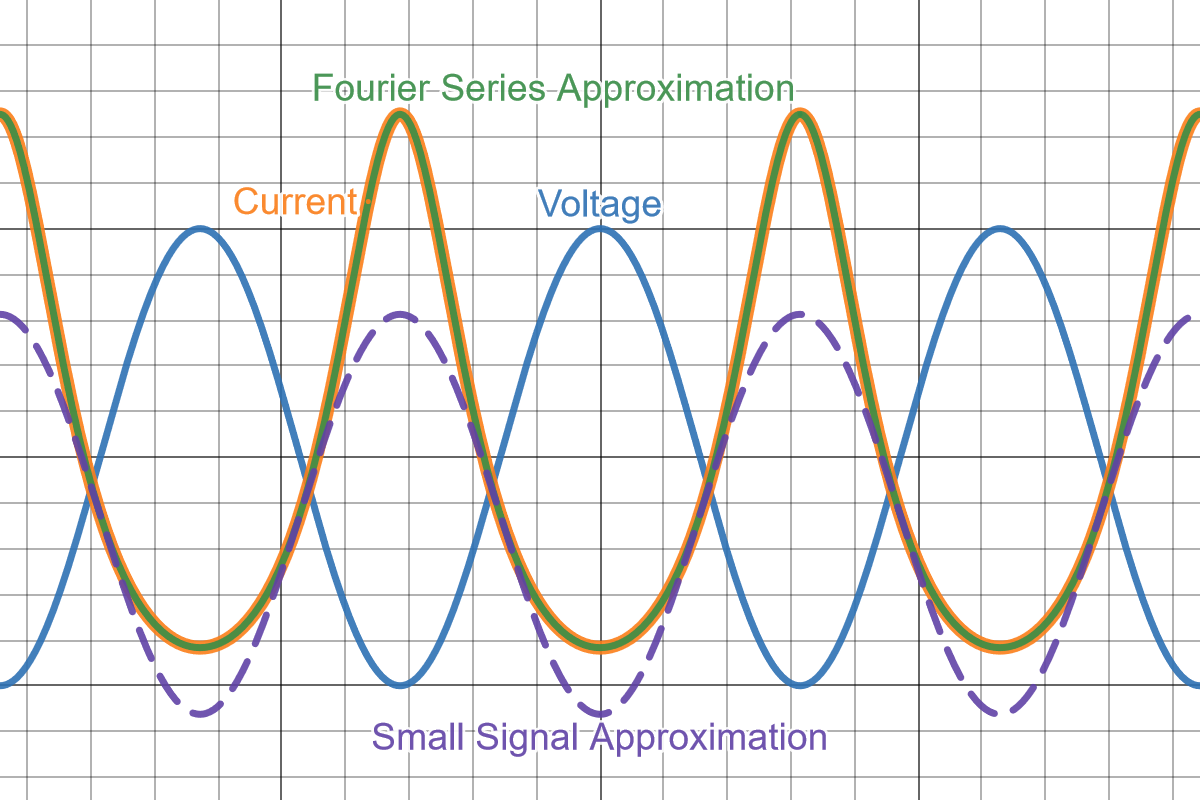
\includegraphics[width=0.5\linewidth]{figs/cpl_fourier_rect.png}
    \caption{Fourier and small signal approximation to constant power load current.}
    \label{fig:results}
\end{figure}



\setcounter{section}{0}
\renewcommand\thesection{\Alph{section}}
\renewcommand\theequation{\Alph{section}.\arabic{equation}}
\section*{Appendix}

\setcounter{equation}{0}
\section{Two Real Pole Functions}

Let $f(z) = z^2 + 2A z + 1$, where $A > 0$, it's poles would be
\begin{IEEEeqnarray}{rCl}
	z_0 &=& -A + \sqrt{A^2 - 1}, \quad \mathrm{and} \\
	z_1 &=& -A - \sqrt{A^2 - 1}. \label{eq:poles}
\end{IEEEeqnarray}

These poles may combined into useful identities:
\begin{IEEEeqnarray}{rCl}
	z_0-z_1 &=& 2\sqrt{A^2 - 1} \label{eq:pole_identity1}, \\
	z_0 z_1 &=& 1 \label{eq:pole_identity2}.
\end{IEEEeqnarray}

Using these identities, and the geometric series of $1/(1-a) = \sum_{k=0}^\infty a^k$, $f(z)$ may be rearranged as follows:
\begin{IEEEeqnarray}{rCl}
f(z)&=& \frac{1}{(z-z_0)(z-z_1)} \nonumber\\
	&=& \cancelToOne{\frac{1}{z_0 z_1}} \frac{1}{\left(1-\frac{z}{z_0}\right)\left(1-\frac{z}{z_1}\right)} \nonumber\\
	&=& \frac{1}{z_0 - z_1}\left(\frac{z_0}{1-\frac{z}{z_1}} - \frac{z_1}{1-\frac{z}{z_0}}\right) \nonumber\\
	&=& \frac{1}{z_0 - z_1}\left(z_0\sum_{k=0}^\infty\left(\frac{z}{z_1}\right)^k - z_1\sum_{k=0}^\infty\left(\frac{z}{z_0}\right)^k\right) \nonumber\\
	&=& \frac{1}{z_0 - z_1}\sum_{k=0}^\infty z^k\left(z_0\left(\frac{1}{z_1}\right)^k - z_1\left(\frac{1}{z_0}\right)^k\right) \nonumber\\
	&=& \frac{1}{z_0 - z_1}\sum_{k=0}^\infty z^k\left(z_0^{k+1} - z_1^{k+1}\right). \label{eq:pole_identity3}
\end{IEEEeqnarray}

\setcounter{equation}{0}
\section{Contour Integrals}

\begin{equation}
\oint z^k dz = 	2 \pi j \mathop{\mathrm{Res}}_{z=0}(z^k) = \begin{cases}
					2\pi j \quad &\text{if} \, k=-1 \\
					0 \quad &\text{otherwise}
				\end{cases}. \label{eq:residue_identity1}
\end{equation}

Using the above, we can create a even more general identity:
\begin{IEEEeqnarray}{rCl}
\oint \sum_{k}^{\infty} a^k z^k dz &=& \sum_{k}^{\infty} \oint  a^kz^k \,dz	\nonumber\\
	&=& \cancelToZero{\sum_{k=-2}^{-\infty}\oint a^{k}z^{k} \,dz} + \oint a^{-1}z^{-1} \,dz + \cancelToZero{\sum_{k=0}^{\infty} \oint a^{k}z^{k} \,dz} \nonumber\\
	&=& \frac{2\pi j}{a} \label{eq:residue_identity2}
\end{IEEEeqnarray}




% \subsection{Pictures}

% \begin{figure}[htbp]
%     \center
%     \includegraphics[scale=0.06]{img/photo.jpg}
%     \caption{Sydney, NSW}
% \end{figure}

% \subsection{Citation}

% This is a citation\cite{Eg}.

\newpage

% ------------------------------------------------------------------------------
% Reference and Cited Works
% ------------------------------------------------------------------------------

\bibliographystyle{IEEEtran}
\begin{thebibliography}{1}

\bibitem{leonard_2014}
J.\@ P.\@ Leonard, ``Nonlinear Modeling Of Dc Constant Power Loads With Frequency Domain Volterra Kernels,''Florida State University, 2014.

\end{thebibliography}
% ------------------------------------------------------------------------------

\end{document}